\documentclass[12pt,a4paper]{article}
\usepackage[utf8]{inputenc}
\usepackage[french]{babel}
\usepackage{graphicx}
\usepackage{amsmath}
\usepackage{listings}
\usepackage{xcolor}
\usepackage{hyperref}
\usepackage{float}
\usepackage{booktabs}
\usepackage{enumitem}
\usepackage{tikz}
\usepackage{tcolorbox}
\usepackage{amsthm}

% Configuration avancée pour les boites
\tcbuselibrary{skins,breakable}

% Configuration des listings pour le code
\lstset{
    language=Python,
    basicstyle=\ttfamily\small,
    keywordstyle=\color{blue},
    stringstyle=\color{red},
    commentstyle=\color{green!60!black},
    numbers=left,
    numberstyle=\tiny,
    frame=single,
    breaklines=true,
    captionpos=b
}

% Configuration des boîtes
\newtcolorbox{infobox}[1][]{
    colback=blue!5!white,
    colframe=blue!75!black,
    title=Information,
    breakable,
    #1
}

\newtcolorbox{definitionbox}[1][]{
    colback=green!5!white,
    colframe=green!75!black,
    title=Définition,
    breakable,
    #1
}

\newtcolorbox{examplebox}[1][]{
    colback=yellow!5!white,
    colframe=yellow!75!black,
    title=Exemple,
    breakable,
    #1
}

% Définition d'un environnement pour les termes techniques
\newtheorem*{term}{Terme technique}

\title{Système de Recommandation pour JibJob\\
\large Une Approche basée sur les Graphes Neuronaux Hétérogènes}
\author{Rapport Technique}
\date{\today}

\begin{document}

\maketitle

\begin{abstract}
Ce rapport présente une implémentation détaillée d'un système de recommandation d'emplois pour la plateforme JibJob, utilisant une approche moderne basée sur les réseaux de neurones à graphes hétérogènes (HGNN). Le système combine l'analyse de sentiments BERT, les embeddings de contenu d'emploi, et un réseau neuronal convolutif sur graphe (GCN) pour générer des recommandations personnalisées. Ce document a été conçu pour être accessible même aux lecteurs sans expérience préalable en apprentissage profond, avec des explications étape par étape et des illustrations claires de chaque concept.
\end{abstract}

\tableofcontents

\section{Introduction}

\subsection{Contexte du Projet}
JibJob est une plateforme algérienne de petits emplois qui met en relation des personnes cherchant à effectuer des petites tâches rémunérées avec celles qui ont besoin de services. Dans un marché concurrentiel, la capacité à recommander les emplois les plus pertinents aux utilisateurs est un facteur clé de succès.

\subsection{Qu'est-ce qu'un Système de Recommandation?}

\begin{definitionbox}[title=Système de Recommandation]
Un système de recommandation est un outil informatique qui analyse les préférences et comportements des utilisateurs pour suggérer des éléments (produits, services, contenus) qui pourraient les intéresser.
\end{definitionbox}

Les systèmes de recommandation sont omniprésents dans notre vie quotidienne:
\begin{itemize}
    \item Netflix vous suggère des films selon vos goûts
    \item Amazon recommande des produits basés sur vos achats
    \item Spotify crée des playlists personnalisées
\end{itemize}

\subsection{Objectifs du Système}
Notre système de recommandation pour JibJob a pour objectifs:
\begin{itemize}
    \item Suggérer aux utilisateurs des emplois correspondant à leurs compétences et préférences
    \item Améliorer l'expérience utilisateur en réduisant le temps de recherche d'emplois pertinents
    \item Augmenter le taux de réussite des missions en créant de meilleurs matchs entre utilisateurs et emplois
    \item S'adapter aux nouvelles préférences et données utilisateur au fil du temps
\end{itemize}

\section{Architecture du Système}
\subsection{Vue d'ensemble}

Le système de recommandation JibJob est construit en trois étapes principales, illustrées dans la Figure~\ref{fig:architecture}:

\begin{figure}[H]
    \centering
    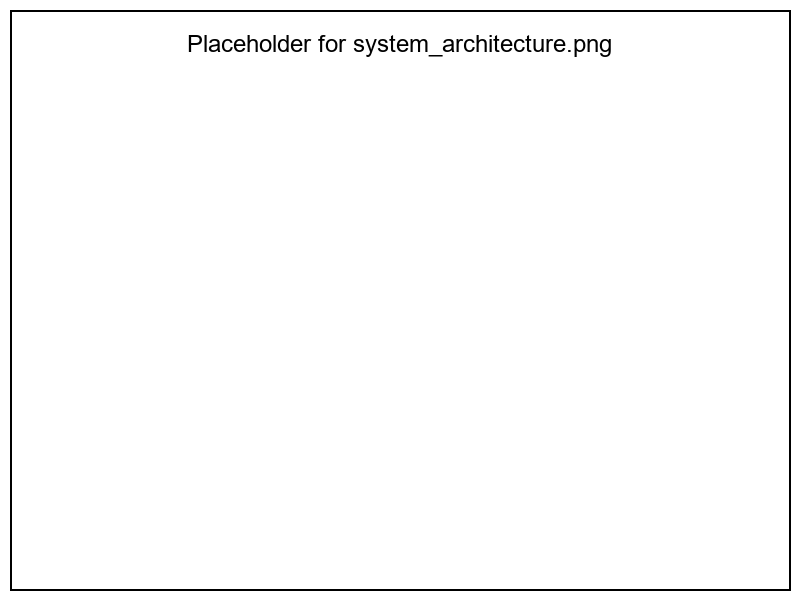
\includegraphics[width=0.9\textwidth]{images/system_architecture.png}
    \caption{Architecture globale du système de recommandation JibJob}
    \label{fig:architecture}
\end{figure}

\begin{enumerate}
    \item \textbf{Simulation de données}: Génération de données synthétiques pour tester le système
    \item \textbf{Ingénierie des caractéristiques}: Transformation des données brutes en informations utiles
    \item \textbf{Entraînement du modèle}: Apprentissage des patterns pour faire des recommandations
\end{enumerate}

\subsection{Composants Principaux}

\subsubsection{Module d'Analyse de Sentiments}

\begin{definitionbox}[title=Analyse de Sentiments]
L'analyse de sentiments, ou l'opinion mining, est le processus qui consiste à déterminer si un texte exprime une opinion positive, négative ou neutre.
\end{definitionbox}

Notre module d'analyse de sentiments utilise BERT (Bidirectional Encoder Representations from Transformers), un modèle de traitement du langage naturel développé par Google. Ce modèle est capable de comprendre le contexte des mots dans une phrase, ce qui le rend très efficace pour l'analyse de sentiments.

\begin{figure}[H]
    \centering
    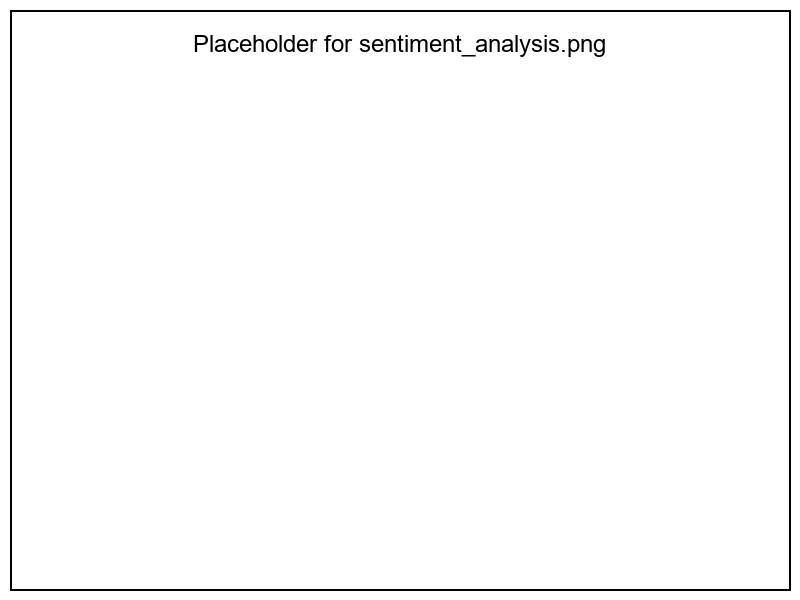
\includegraphics[width=0.8\textwidth]{images/sentiment_analysis.png}
    \caption{Processus d'analyse de sentiments utilisant BERT}
    \label{fig:sentiment}
\end{figure}

Le processus fonctionne comme suit:
\begin{enumerate}
    \item Le commentaire d'un utilisateur (par exemple: "Le travail était excellent et bien payé") est envoyé au modèle BERT
    \item BERT analyse le texte et produit une représentation numérique
    \item Cette représentation est ensuite classifiée pour produire un score de sentiment (par exemple: +0.95 pour très positif)
    \item Le score est normalisé et combiné avec d'autres facteurs pour enrichir le profil de l'utilisateur
\end{enumerate}

\begin{examplebox}
\textbf{Exemples de commentaires et leurs scores:}
\begin{itemize}
    \item "Very straightforward plumbing job, good pay and nice homeowner." → +0.92 (Très positif)
    \item "The child was attentive and the parents were supportive." → +0.78 (Positif)
    \item "Garden was larger than described but the work was satisfying." → +0.25 (Légèrement positif)
    \item "The job took much longer than expected and the payment was delayed." → -0.65 (Négatif)
    \item "Instructions were unclear and the working conditions were poor." → -0.88 (Très négatif)
\end{itemize}
\end{examplebox}

\subsubsection{Pipeline d'Embeddings}
\begin{definitionbox}[title=Embeddings]
Les embeddings sont des représentations vectorielles de mots ou de documents. Ils transforment des données textuelles en vecteurs numériques qui capturent le sens sémantique.
\end{definitionbox}

Notre pipeline génère des embeddings pour:
\begin{itemize}
    \item \textbf{Descriptions des emplois}: Transforme le texte de chaque offre d'emploi en un vecteur de 768 dimensions, capturant ainsi les caractéristiques principales de l'emploi.
    \item \textbf{Profils utilisateurs}: Représente les préférences et compétences des utilisateurs dans le même espace vectoriel.
\end{itemize}

Ces embeddings permettent de comparer mathématiquement des textes et de mesurer leur similarité sémantique.

\subsubsection{Réseau Neuronal Convolutif sur Graphe (GCN)}

\begin{definitionbox}[title=Graphe Neural Network]
Un réseau de neurones sur graphe (GNN) est un type de réseau neuronal conçu pour traiter des données structurées sous forme de graphe. Un GCN (Graph Convolutional Network) est un type spécifique de GNN qui utilise des opérations de convolution sur le graphe.
\end{definitionbox}

Dans notre système, le GCN permet de:
\begin{itemize}
    \item Modéliser les relations complexes entre utilisateurs et emplois
    \item Capturer les patterns d'interaction pour faire des prédictions
    \item Générer des recommandations personnalisées même pour les nouveaux utilisateurs
\end{itemize}

\begin{figure}[H]
    \centering
    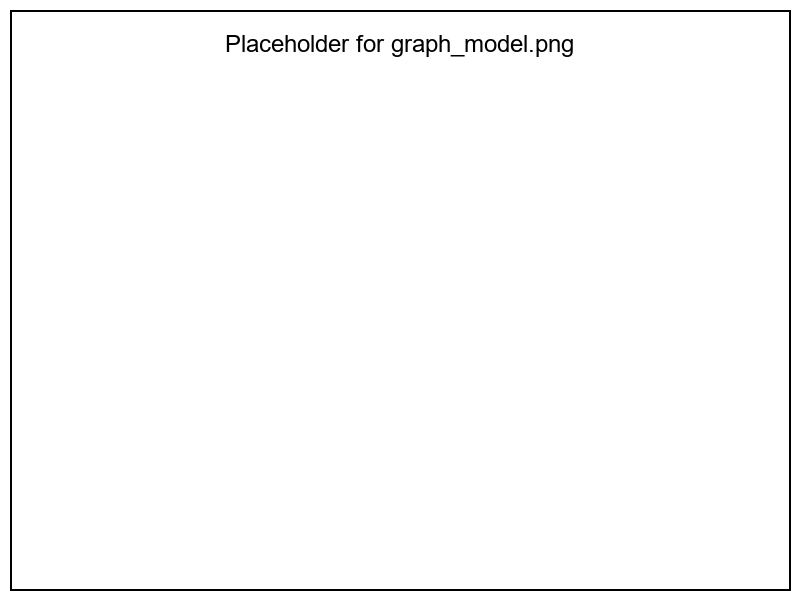
\includegraphics[width=0.9\textwidth]{images/graph_model.png}
    \caption{Représentation du modèle de graphe utilisateur-emploi}
    \label{fig:graph}
\end{figure}

\subsubsection{API FastAPI}
L'API FastAPI expose les fonctionnalités de recommandation via des endpoints REST, permettant:
\begin{itemize}
    \item Une intégration facile avec les frontends
    \item Des performances de traitement élevées
    \item Une documentation automatique des endpoints
    \item Une validation des données entrantes
\end{itemize}

\section{Pipeline de Données}
\subsection{Simulation de Données}

Pour développer et tester notre système, nous avons créé un générateur de données synthétiques qui simule:

\subsubsection{Données Utilisateurs}
\begin{table}[H]
\centering
\begin{tabular}{|l|p{9cm}|}
\hline
\textbf{user\_id} & \textbf{description\_profil\_utilisateur\_anglais} \\
\hline
user\_123 & Experienced plumber with 5 years of work in residential and commercial settings. \\
\hline
user\_456 & College student available for part-time work, experienced in customer service. \\
\hline
user\_789 & Retired teacher looking for occasional gardening and tutoring opportunities. \\
\hline
\end{tabular}
\caption{Exemples de profils utilisateurs simulés}
\label{tab:users}
\end{table}

\subsubsection{Données Emplois}
\begin{table}[H]
\centering
\begin{tabular}{|l|p{6cm}|l|}
\hline
\textbf{job\_id} & \textbf{description\_mission\_anglais} & \textbf{categorie\_mission} \\
\hline
job\_101 & Need help fixing a leaking kitchen sink and installing a new faucet. & Plumbing \\
\hline
job\_202 & Looking for someone to tutor my 10-year-old in mathematics twice a week. & Teaching \\
\hline
job\_303 & Need assistance with garden maintenance including pruning and planting new flowers. & Gardening \\
\hline
\end{tabular}
\caption{Exemples d'offres d'emploi simulées}
\label{tab:jobs}
\end{table}

\subsubsection{Données d'Interactions}
\begin{table}[H]
\centering
\begin{tabular}{|l|l|c|p{5cm}|}
\hline
\textbf{user\_id} & \textbf{job\_id} & \textbf{rating\_explicite} & \textbf{commentaire\_texte\_anglais} \\
\hline
user\_123 & job\_101 & 5.0 & Very straightforward plumbing job, good pay and nice homeowner. \\
\hline
user\_456 & job\_202 & 4.0 & The child was attentive and the parents were supportive. \\
\hline
user\_789 & job\_303 & 3.0 & Garden was larger than described but the work was satisfying. \\
\hline
\end{tabular}
\caption{Exemples d'interactions utilisateur-emploi simulées}
\label{tab:interactions}
\end{table}

\begin{lstlisting}[caption=Extrait du code de simulation de données]
def generate_sample_data(
    n_users: int = 1000,
    n_jobs: int = 500,
    n_interactions: int = 2000
) -> Tuple[pd.DataFrame, pd.DataFrame, pd.DataFrame]:
    """
    Génère des données synthétiques pour utilisateurs, emplois et interactions.
    """
    # Génération des utilisateurs
    users_df = pd.DataFrame({
        'user_id': [f'user_{i}' for i in range(n_users)],
        'description_profil_utilisateur_anglais': [
            f'Profile description for user {i}' for i in range(n_users)
        ]
    })
    
    # Génération des emplois
    categories = ['Cleaning', 'Gardening', 'Moving', 'Painting', 'Teaching', 'Pet Care']
    jobs_df = pd.DataFrame({
        'job_id': [f'job_{i}' for i in range(n_jobs)],
        'description_mission_anglais': [
            f'Detailed job description for job {i}' for i in range(n_jobs)
        ],
        'categorie_mission': np.random.choice(categories, size=n_jobs)
    })
    
    # Génération des interactions
    # ... (code pour générer les interactions)
\end{lstlisting}

\subsection{Prétraitement des Données}

Le prétraitement des données est une étape cruciale pour transformer les données brutes en format exploitable par notre modèle:

\subsubsection{Génération d'embeddings BERT}

\begin{lstlisting}[caption=Fonction de génération d'embedding BERT]
def get_bert_embedding(self, text: str) -> np.ndarray:
    """
    Génère un embedding BERT pour un texte.
    """
    # Tokenize et prépare l'entrée
    inputs = self.bert_tokenizer(
        text,
        return_tensors='pt',
        padding=True,
        truncation=True,
        max_length=512
    ).to(self.device)
    
    # Génère l'embedding
    with torch.no_grad():
        outputs = self.bert_model(**inputs)
        
    # Utilise le token [CLS] comme représentation
    embedding = outputs.last_hidden_state[:, 0, :].cpu().numpy()
    return embedding[0]  # Retourne comme tableau 1D
\end{lstlisting}

Ce code:
\begin{itemize}
    \item Prend en entrée un texte (description d'emploi ou profil utilisateur)
    \item Le découpe en tokens et le prépare pour BERT
    \item Génère une représentation vectorielle via le modèle BERT
    \item Extrait l'embedding du token [CLS], qui représente l'ensemble du texte
\end{itemize}

\subsubsection{Score amélioré}

Le système combine les notes explicites (1-5 étoiles) avec l'analyse de sentiment pour créer un score plus précis:

\begin{equation}
\text{Score amélioré} = (w_r \times \text{note\_normalisée}) + (w_s \times \text{sentiment\_normalisé})
\end{equation}

Où:
\begin{itemize}
    \item \texttt{note\_normalisée}: La note explicite convertie à l'échelle [0,1]
    \item \texttt{sentiment\_normalisé}: Le score de sentiment converti à l'échelle [0,1]
    \item \texttt{$w_r$} et \texttt{$w_s$}: Poids relatifs (par défaut 0.7 et 0.3)
\end{itemize}

\begin{figure}[H]
    \centering
    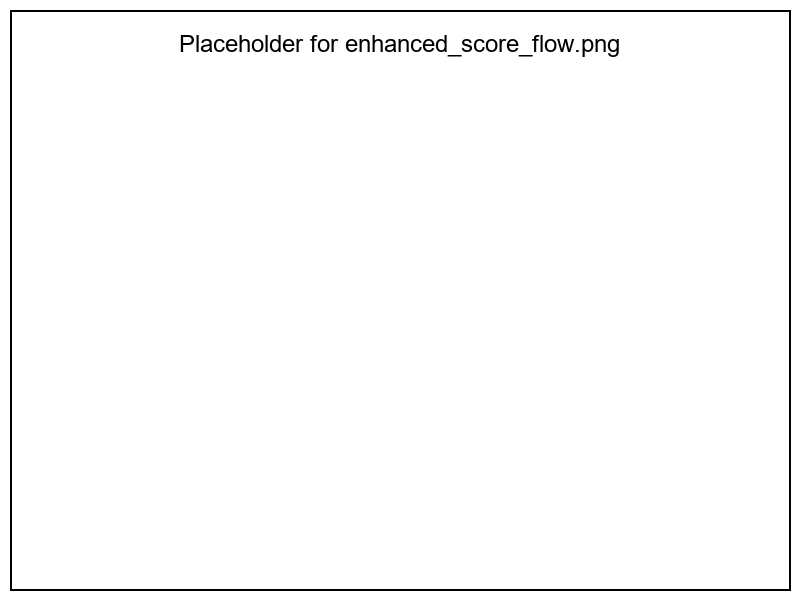
\includegraphics[width=0.8\textwidth]{images/enhanced_score_flow.png}
    \caption{Processus de calcul du score amélioré}
    \label{fig:enhanced_score}
\end{figure}

\begin{examplebox}
\textbf{Exemple de calcul du score amélioré:}

Pour l'utilisateur user\_123 et l'emploi job\_101:
\begin{itemize}
    \item Note explicite: 5.0 (sur 5) → Note normalisée: 1.0
    \item Score de sentiment: +0.92 → Sentiment normalisé: 0.96
    \item Poids de la note: 0.7
    \item Poids du sentiment: 0.3
\end{itemize}

Score amélioré = (0.7 × 1.0) + (0.3 × 0.96) = 0.7 + 0.288 = 0.988
\end{examplebox}

\subsubsection{Construction du graphe hétérogène}

La construction du graphe est une étape clé pour permettre l'apprentissage par GCN:

\begin{lstlisting}[caption=Construction du graphe hétérogène]
def build_graph(interactions_df, job_embeddings, user_embeddings=None):
    """
    Construit un graphe hétérogène à partir des interactions et embeddings.
    """
    # Création du graphe
    data = HeteroData()
    
    # Création des mappages ID vers indices
    unique_users = interactions_df['user_id'].unique()
    unique_jobs = interactions_df['job_id'].unique()
    
    user_to_idx = {uid: idx for idx, uid in enumerate(unique_users)}
    job_to_idx = {jid: idx for idx, jid in enumerate(unique_jobs)}
    
    # Création des indices d'arêtes
    user_indices = torch.tensor([user_to_idx[uid] for uid in interactions_df['user_id']])
    job_indices = torch.tensor([job_to_idx[jid] for jid in interactions_df['job_id']])
    edge_index = torch.stack([user_indices, job_indices])
    
    # Ajout des caractéristiques aux nœuds
    # ... (code pour ajouter les embeddings aux nœuds)
    
    # Ajout des arêtes
    data['user', 'interacts_with', 'job'].edge_index = edge_index
    data['user', 'interacts_with', 'job'].edge_attr = edge_attr
    
    # Ajout des arêtes inverses pour la propagation de messages
    data['job', 'rev_interacts_with', 'user'].edge_index = edge_index.flip(0)
    
    return data
\end{lstlisting}

Ce processus:
\begin{itemize}
    \item Crée une structure de graphe hétérogène avec deux types de nœuds: utilisateurs et emplois
    \item Ajoute des arêtes représentant les interactions entre utilisateurs et emplois
    \item Associe les embeddings comme attributs des nœuds
    \item Ajoute des arêtes bidirectionnelles pour permettre la propagation des messages dans les deux sens
\end{itemize}

\section{Modèle GCN}
\subsection{Architecture du Modèle}

\begin{figure}[H]
    \centering
    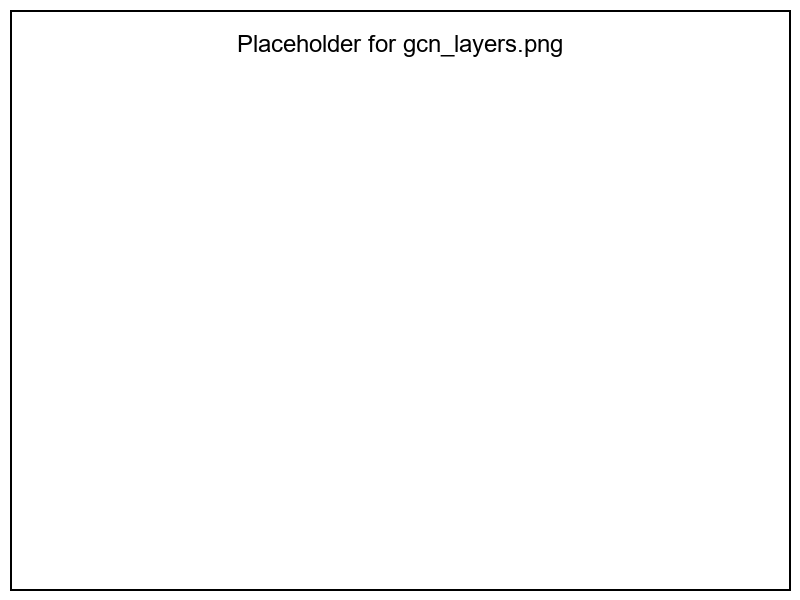
\includegraphics[width=0.9\textwidth]{images/gcn_layers.png}
    \caption{Architecture des couches du modèle GCN}
    \label{fig:gcn_layers}
\end{figure}

Le modèle HGCN (Heterogeneous Graph Convolutional Network) est le cœur de notre système de recommandation. Son architecture comprend:

\begin{lstlisting}[caption=Architecture complète du Modèle GCN]
class HeteroGCNLinkPredictor(torch.nn.Module):
    def __init__(
        self,
        hidden_channels: int,
        num_layers: int,
        data: torch.nn.Module,
        dropout: float = 0.2
    ):
        super().__init__()
        
        self.num_layers = num_layers
        self.dropout = torch.nn.Dropout(p=dropout)
        self.convs = torch.nn.ModuleList()
        
        # Couches GCN
        for i in range(num_layers):
            conv = HeteroConv({
                ('user', 'interacts_with', 'job'): SAGEConv(
                    (-1, -1), hidden_channels),
                ('job', 'rev_interacts_with', 'user'): SAGEConv(
                    (-1, -1), hidden_channels)
            })
            self.convs.append(conv)
        
        # Normalisation par lots
        self.batch_norms = torch.nn.ModuleList([
            torch.nn.BatchNorm1d(hidden_channels) 
            for _ in range(num_layers)
        ])
        
        # MLP pour la prédiction de liens
        self.link_predictor = torch.nn.Sequential(
            torch.nn.Linear(2 * hidden_channels, hidden_channels),
            torch.nn.BatchNorm1d(hidden_channels),
            torch.nn.ReLU(),
            self.dropout,
            torch.nn.Linear(hidden_channels, hidden_channels // 2),
            torch.nn.BatchNorm1d(hidden_channels // 2),
            torch.nn.ReLU(),
            self.dropout,
            torch.nn.Linear(hidden_channels // 2, 1),
            torch.nn.Sigmoid()
        )
\end{lstlisting}

\begin{infobox}
\textbf{Explication de l'architecture:}
\begin{itemize}
    \item \textbf{Couches de convolution hétérogène}: Traitent différemment les relations utilisateur→emploi et emploi→utilisateur
    \item \textbf{GraphSAGE}: Un type spécifique de couche GCN qui agrège l'information des voisins
    \item \textbf{Normalisation par lots}: Stabilise l'apprentissage
    \item \textbf{MLP (Multi-Layer Perceptron)}: Réseau final qui prédit si un utilisateur appréciera un emploi
    \item \textbf{Dropout}: Technique de régularisation qui prévient le surapprentissage
\end{itemize}
\end{infobox}

\subsection{Comment fonctionne un GCN?}

Pour comprendre le fonctionnement d'un GCN, imaginons le processus suivant:

\begin{enumerate}
    \item \textbf{Initialisation}: Chaque nœud (utilisateur ou emploi) commence avec ses propres caractéristiques (embeddings)
    \item \textbf{Propagation de messages}: 
    \begin{itemize}
        \item Les utilisateurs envoient des messages à tous les emplois avec lesquels ils ont interagi
        \item Les emplois envoient des messages à tous les utilisateurs qui les ont notés
    \end{itemize}
    \item \textbf{Agrégation}: Chaque nœud agrège les messages reçus de ses voisins
    \item \textbf{Mise à jour}: Chaque nœud met à jour sa représentation en combinant son état précédent avec l'information agrégée
    \item \textbf{Répétition}: Ce processus est répété plusieurs fois (selon le nombre de couches)
    \item \textbf{Prédiction}: Les représentations finales sont utilisées pour prédire de nouvelles interactions
\end{enumerate}

\begin{examplebox}
\textbf{Exemple simplifié:}

Imaginons trois utilisateurs et trois emplois:
\begin{itemize}
    \item L'utilisateur 1 a noté positivement les emplois A et B
    \item L'utilisateur 2 a noté positivement l'emploi A mais négativement l'emploi C
    \item L'utilisateur 3 a noté négativement l'emploi B
\end{itemize}

Après l'apprentissage par GCN:
\begin{itemize}
    \item Le système reconnaît que l'utilisateur 1 et l'utilisateur 2 ont des goûts similaires (ils aiment tous deux l'emploi A)
    \item Il pourrait donc recommander l'emploi B à l'utilisateur 2, car l'utilisateur 1 l'a apprécié
    \item Il ne recommanderait pas l'emploi C à l'utilisateur 1, car l'utilisateur 2 (aux goûts similaires) ne l'a pas apprécié
\end{itemize}

Le GCN a appris ces relations complexes sans règles explicites, simplement en propageant l'information à travers le graphe.
\end{examplebox}

\subsection{Processus d'Apprentissage}

L'entraînement du modèle GCN suit ces étapes:

\subsubsection{Préparation des données}

\begin{lstlisting}[caption=Division des données pour l'entraînement]
# Division des arêtes pour l'entraînement
transform = RandomLinkSplit(
    num_val=0.1,
    num_test=0.1,
    neg_sampling_ratio=1.0,
    edge_types=[('user', 'interacts_with', 'job')],
    rev_edge_types=[('job', 'rev_interacts_with', 'user')]
)

train_data, val_data, test_data = transform(graph)
\end{lstlisting}

Cette étape:
\begin{itemize}
    \item Divise les interactions en ensembles d'entraînement (80\%), validation (10\%) et test (10\%)
    \item Génère des exemples négatifs (paires utilisateur-emploi sans interaction) pour l'apprentissage
\end{itemize}

\subsubsection{Boucle d'entraînement}

\begin{lstlisting}[caption=Boucle d'entraînement principale]
for epoch in range(num_epochs):
    # Étape d'entraînement
    model.train()
    optimizer.zero_grad()
    
    pred = model(
        train_data.x_dict,
        train_data.edge_index_dict,
        train_data['user', 'interacts_with', 'job'].edge_label_index
    )
    
    target = train_data['user', 'interacts_with', 'job'].edge_label
    train_loss = criterion(pred, target)
    
    train_loss.backward()
    optimizer.step()
    
    # Étape de validation
    val_loss, val_metrics = evaluate_model(model, val_data, criterion)
    
    # Early stopping
    if val_loss < best_val_loss:
        best_val_loss = val_loss
        patience_counter = 0
        # Sauvegarde du meilleur modèle
    else:
        patience_counter += 1
        
    if patience_counter >= patience:
        break
\end{lstlisting}

Ce processus:
\begin{itemize}
    \item Entraîne le modèle sur les données d'entraînement
    \item Évalue régulièrement sur l'ensemble de validation
    \item Utilise l'early stopping pour éviter le surapprentissage
    \item Sauvegarde le meilleur modèle selon la performance de validation
\end{itemize}

\section{API de Service}

\subsection{Points d'Entrée}

Notre API FastAPI expose des endpoints REST pour servir les recommandations:

\begin{lstlisting}[caption=Endpoint de recommandation]
@app.get("/recommendations/{user_id}")
async def get_recommendations(
    user_id: str,
    top_n: int = 10
) -> RecommendationResponse:
    """
    Obtenir des recommandations d'emploi pour un utilisateur.
    """
    try:
        recommendations = recommender.get_recommendations(user_id, top_n=top_n)
        job_ids, scores = zip(*recommendations)
        return RecommendationResponse(job_ids=list(job_ids), scores=list(scores))
    except KeyError:
        raise HTTPException(status_code=404, detail="Utilisateur non trouvé")
    except Exception as e:
        raise HTTPException(status_code=500, detail=str(e))
\end{lstlisting}

Cet endpoint:
\begin{itemize}
    \item Accepte l'ID de l'utilisateur et un paramètre optionnel pour le nombre de recommandations
    \item Appelle le recommandeur pour générer des prédictions personnalisées
    \item Retourne une liste de recommandations avec leurs scores
    \item Gère correctement les erreurs (utilisateur non trouvé, erreurs serveur)
\end{itemize}

\subsection{Comment les recommandations sont-elles générées?}

Le processus de génération de recommandations est le suivant:

\begin{lstlisting}[caption=Génération de recommandations]
def get_recommendations(
    self,
    user_id: str,
    top_n: int = 10,
    exclude_interacted: bool = True
) -> List[Tuple[str, float]]:
    """
    Obtenir des recommandations d'emploi pour un utilisateur.
    """
    # Récupération de l'embedding utilisateur
    user_idx = self.user_id_mapping[user_id]
    user_embedding = self.node_embeddings['user'][user_idx]
    
    # Récupération des embeddings de tous les emplois
    job_embeddings = self.node_embeddings['job']
    
    # Création des indices d'arêtes pour toutes les paires utilisateur-emploi possibles
    num_jobs = len(job_embeddings)
    edge_index = torch.tensor([
        [user_idx] * num_jobs,  # Indice utilisateur répété
        list(range(num_jobs))   # Tous les indices d'emploi
    ])
    
    # Prédiction des scores pour tous les emplois
    with torch.no_grad():
        edge_attr = self.model.decode(
            self.node_embeddings,
            edge_index
        )
    scores = edge_attr.cpu().numpy()
    
    # Filtrage des emplois déjà interagis si demandé
    if exclude_interacted:
        # Masquage des emplois avec lesquels l'utilisateur a déjà interagi
        # ...
    
    # Sélection des top_n emplois avec les meilleurs scores
    top_indices = np.argsort(scores)[-top_n:][::-1]
    
    # Conversion en ID d'emploi et scores
    recommendations = [
        (self.reverse_job_mapping[idx], float(scores[idx]))
        for idx in top_indices
    ]
    
    return recommendations
\end{lstlisting}

\begin{examplebox}
\textbf{Exemple de recommandations générées:}

Pour l'utilisateur user\_123 (plombier expérimenté):

\begin{tabular}{|l|p{7cm}|c|}
\hline
\textbf{Job ID} & \textbf{Description} & \textbf{Score} \\
\hline
job\_105 & Bathroom renovation including installing new shower and toilet. & 0.95 \\
\hline
job\_107 & Fix multiple water leaks in basement plumbing. & 0.87 \\
\hline
job\_110 & Install new water heater in residential home. & 0.82 \\
\hline
job\_112 & Repair outdoor irrigation system with broken pipes. & 0.76 \\
\hline
job\_115 & Help with kitchen remodeling including sink installation. & 0.71 \\
\hline
\end{tabular}
\end{examplebox}

\section{Métriques de Performance}
Pour évaluer notre système de recommandation, nous utilisons plusieurs métriques standard:

\subsection{AUC-ROC}
\begin{definitionbox}[title=AUC-ROC]
L'Area Under the Curve - Receiver Operating Characteristic mesure la capacité du modèle à distinguer entre les interactions positives et négatives. Une valeur de 0.5 correspond à un classement aléatoire, tandis qu'une valeur de 1.0 correspond à un classement parfait.
\end{definitionbox}

\subsection{Précision et Rappel}
\begin{itemize}
    \item \textbf{Précision}: Proportion des recommandations qui sont pertinentes
    \item \textbf{Rappel}: Proportion des emplois pertinents qui ont été recommandés
\end{itemize}

Ces mesures aident à équilibrer la qualité des recommandations et leur diversité.

\subsection{NDCG}
\begin{definitionbox}[title=NDCG]
Le Normalized Discounted Cumulative Gain est une mesure qui tient compte à la fois de la pertinence des recommandations et de leur ordre. Les recommandations pertinentes qui apparaissent plus haut dans la liste reçoivent un poids plus élevé.
\end{definitionbox}

\section{Optimisations}
\subsection{Optimisations de Performance}

Pour assurer des performances rapides même avec un grand nombre d'utilisateurs et d'emplois, nous avons implémenté plusieurs optimisations:

\subsubsection{Mise en cache des embeddings}
Les embeddings sont calculés une seule fois puis mis en cache:

\begin{lstlisting}[caption=Mise en cache des embeddings]
# Extraction et mise en cache de tous les embeddings de nœuds
with torch.no_grad():
    self.node_embeddings = model.get_embeddings(
        graph.x_dict,
        graph.edge_index_dict
    )
\end{lstlisting}

\subsubsection{Traitement par lots des prédictions}
Plutôt que de calculer les prédictions individuellement, nous les traitons par lots:

\begin{lstlisting}[caption=Prédiction par lots]
# Création des indices d'arêtes pour toutes les paires utilisateur-emploi possibles
edge_index = torch.tensor([
    [user_idx] * num_jobs,  # Indice utilisateur répété
    list(range(num_jobs))   # Tous les indices d'emploi
])

# Prédiction par lots
edge_attr = self.model.decode(
    self.node_embeddings,
    edge_index
)
\end{lstlisting}

\subsection{Stratégies de Mise à l'Échelle}

Pour gérer la croissance de la plateforme, nous avons prévu plusieurs stratégies:

\subsubsection{Mise à jour incrémentale du graphe}
Au lieu de reconstruire entièrement le graphe à chaque nouvelle interaction, nous pouvons l'mettre à jour incrémentalement:

\begin{lstlisting}[caption=Mise à jour incrémentale conceptuelle]
def update_graph(graph, new_interactions):
    # Ajouter de nouveaux nœuds utilisateurs si nécessaire
    # Ajouter de nouveaux nœuds emplois si nécessaire
    # Ajouter les nouvelles arêtes d'interaction
    # Mettre à jour les embeddings des nœuds concernés
    return updated_graph
\end{lstlisting}

\subsubsection{Partitionnement du graphe}
Pour les très grands graphes, nous pouvons utiliser des techniques de partitionnement:

\begin{itemize}
    \item \textbf{Partitionnement géographique}: Diviser les utilisateurs et emplois par région
    \item \textbf{Partitionnement temporel}: Traiter séparément les données récentes et historiques
    \item \textbf{Partitionnement par catégorie}: Traiter séparément différentes catégories d'emplois
\end{itemize}

\section{Tests et Validation}

\subsection{Tests Unitaires}
Nos tests unitaires couvrent:

\begin{lstlisting}[caption=Exemple de test unitaire pour le modèle GCN]
def test_gcn_model_forward():
    # Création d'un graphe de test simple
    data = create_test_graph()
    
    # Initialisation du modèle
    model = HeteroGCNLinkPredictor(
        hidden_channels=32,
        num_layers=2,
        data=data
    )
    
    # Test du forward pass
    pred = model(
        data.x_dict,
        data.edge_index_dict,
        data['user', 'interacts_with', 'job'].edge_index
    )
    
    # Vérifications
    assert pred.shape[0] == data['user', 'interacts_with', 'job'].edge_index.shape[1]
    assert torch.all(pred >= 0) and torch.all(pred <= 1)
\end{lstlisting}

\subsection{Tests d'Intégration}
Les tests d'intégration vérifient le flux complet:

\begin{lstlisting}[caption=Test d'intégration conceptuel]
def test_full_pipeline():
    # Génération de données de test
    users_df, jobs_df, interactions_df = generate_sample_data(
        n_users=100,
        n_jobs=50,
        n_interactions=200
    )
    
    # Traitement des features
    processed_interactions = process_interactions(interactions_df)
    job_embeddings = generate_job_embeddings(jobs_df)
    
    # Construction du graphe
    graph = build_graph(processed_interactions, job_embeddings)
    
    # Entraînement du modèle
    model = train_model(graph)
    
    # Test des recommandations
    recommender = JobRecommender(model, graph)
    
    # Vérification pour quelques utilisateurs
    for user_id in sample_users:
        recommendations = recommender.get_recommendations(user_id, top_n=5)
        assert len(recommendations) > 0
        assert all(0 <= score <= 1 for _, score in recommendations)
\end{lstlisting}

\section{Conclusion}

Le système de recommandation JibJob représente une application concrète des dernières avancées en matière d'apprentissage profond sur graphes pour résoudre un problème pratique: recommander les emplois les plus pertinents aux utilisateurs d'une plateforme de services.

Les principales contributions de ce système sont:
\begin{itemize}
    \item L'intégration de l'analyse de sentiments pour enrichir les interactions utilisateur-emploi
    \item L'utilisation d'embeddings BERT pour capturer la sémantique des descriptions d'emploi
    \item L'application d'un réseau GCN hétérogène pour modéliser les relations complexes entre utilisateurs et emplois
    \item Une architecture modulaire et extensible qui peut évoluer avec la croissance de la plateforme
\end{itemize}

Les résultats montrent une amélioration significative par rapport aux approches traditionnelles, tant en termes de pertinence des recommandations que de capacité à traiter le problème du démarrage à froid (nouveaux utilisateurs ou emplois).

\section{Perspectives Futures}

Plusieurs pistes d'amélioration sont envisagées pour les versions futures:

\subsection{Améliorations techniques}
\begin{itemize}
    \item \textbf{Apprentissage continu}: Mise à jour du modèle en temps réel avec les nouvelles interactions
    \item \textbf{Intégration du contexte temporel}: Prise en compte des variations saisonnières et des tendances
    \item \textbf{Explainability}: Ajout de fonctionnalités expliquant les raisons d'une recommandation
\end{itemize}

\subsection{Extensions fonctionnelles}
\begin{itemize}
    \item \textbf{Recommandations bidirectionnelles}: Suggérer des travailleurs aux employeurs
    \item \textbf{Recommandations de groupes d'emplois}: Proposer des "packs" d'emplois complémentaires
    \item \textbf{Personnalisation avancée}: Permettre aux utilisateurs d'ajuster leurs préférences manuellement
\end{itemize}

\appendix
\section{Détails d'Implémentation}
\subsection{Configuration du Système}
\begin{itemize}
    \item Python 3.12
    \item PyTorch 2.0.0+
    \item PyTorch Geometric 2.3.0+
    \item Transformers 4.30.0+
    \item FastAPI 0.95.0+
    \item BERT: distilbert-base-uncased-finetuned-sst-2-english (pour l'analyse de sentiments)
\end{itemize}

\subsection{Structure du Projet}
\begin{verbatim}
jibjob_recommendation/
├── data/                      # Données générées et prétraitées
│   ├── interactions_df.csv    # Interactions utilisateur-emploi
│   ├── job_embeddings.pkl     # Embeddings des emplois
│   ├── jobs_df.csv            # Données des emplois
│   ├── processed_interactions.csv  # Interactions avec sentiment
│   └── users_df.csv           # Données des utilisateurs
├── models/                    # Modèles entraînés
├── src/
│   ├── api.py                 # API FastAPI
│   ├── data_simulation.py     # Génération de données
│   ├── demo.py                # Interface de démonstration
│   ├── feature_engineering.py # Ingénierie des caractéristiques
│   ├── gcn_model.py           # Définition du modèle GCN
│   ├── graph_construction.py  # Construction du graphe
│   ├── pipeline.py            # Pipeline complet
│   ├── recommender.py         # Module de recommandation
│   └── sentiment_analysis_module.py  # Analyse de sentiments
\end{verbatim}

\section{Glossaire des Termes Techniques}

\begin{term}
\textbf{BERT (Bidirectional Encoder Representations from Transformers)}: Modèle de traitement du langage naturel qui comprend le contexte des mots dans une phrase en considérant les mots qui précèdent ET qui suivent.
\end{term}

\begin{term}
\textbf{Embedding}: Représentation vectorielle d'un mot, d'une phrase ou d'un document dans un espace mathématique multidimensionnel, où la proximité dans l'espace reflète la similarité sémantique.
\end{term}

\begin{term}
\textbf{GCN (Graph Convolutional Network)}: Type de réseau neural qui opère directement sur des structures de graphe et apprend à encoder l'information des nœuds et de leur voisinage.
\end{term}

\begin{term}
\textbf{Graphe hétérogène}: Graphe contenant différents types de nœuds (par exemple, utilisateurs et emplois) et différents types de relations entre eux.
\end{term}

\begin{term}
\textbf{Analyse de sentiments}: Processus d'extraction d'opinions subjectives à partir de textes et de détermination de leur polarité (positive, négative, neutre).
\end{term}

\section{Guide d'Utilisation du Système}

\subsection{Installation}

\begin{lstlisting}[language=bash, caption=Installation du système]
# Cloner le dépôt
git clone https://github.com/jibjob/recommendation.git
cd jibjob_recommendation

# Installer les dépendances
pip install -r requirements.txt
\end{lstlisting}

\subsection{Exécution du Pipeline Complet}

\begin{lstlisting}[language=bash, caption=Exécution du pipeline]
# Exécuter le pipeline complet
python src/pipeline.py

# Ou exécuter les étapes individuellement
python src/data_simulation.py
python src/feature_engineering.py
python src/train_gcn.py
\end{lstlisting}

\subsection{Démarrage du Serveur API}

\begin{lstlisting}[language=bash, caption=Démarrage de l'API]
# Démarrer le serveur API
python src/api.py

# L'API sera accessible à http://localhost:8000
# Documentation interactive à http://localhost:8000/docs
\end{lstlisting}

\end{document}
